%---------------DOCUMENT SETTINGS------------------------------------
%\documentclass[headheight=30pt]{scrartcl}
\documentclass{article}

\usepackage[utf8]{inputenc} % utf8x durch utf8 ersetzt wegen biblatex
\usepackage[T1]{fontenc}
\usepackage{amsmath,amssymb,amstext,amsfonts}
\usepackage[ngerman]{babel}
\usepackage{csquotes}
\usepackage{pdfpages} %zum importieren des Deckblattes
\usepackage{geometry}
\usepackage[headsepline]{scrlayer-scrpage}
\usepackage{lastpage}
\usepackage[style=numeric]{biblatex} %Literaturverwaltung
\usepackage{tabularx} %für die Legende im Gruundlagen Oszi Bild
\usepackage{float}
\usepackage{textcomp}
\usepackage{gensymb}
\usepackage{stmaryrd}
\usepackage{graphicx}
\usepackage[export]{adjustbox}
\usepackage{a4wide}
\usepackage{hyperref}
\usepackage{multicol}
\usepackage{makecell}
\usepackage{enumitem}
\usepackage{subcaption}


\geometry{      %holt mehr aus einer A4 Seite raus
    a4paper,
    total={170mm,257mm},
    left=20mm,
    top=15mm,
   }
\graphicspath{ {./graphics/} }  %pfad für bilder
\hypersetup{colorlinks=false}
\addbibresource{literatur.bib} %Literatur-Resourcen\s
%\setlength{\headheight}{0.0pt} % macht zwar headheight warnings aber dafür nutz latex die seitengröße besser aus.
\pagestyle{empty}


\newcommand{\subf}[2]{
    {
        \begin{tabular}[c]{@{}c@{}}
            {\setlength{\extrarowheight}{100pt} #1 }\\#2
        \end{tabular}
    }
}
\newcommand{\allc}{\multicolumn{1}{c|}{-}}
\newcommand{\monofig}[4]{
    
    \begin{figure}[H]
    \centering
    \includegraphics[#1]{#2}
    \caption{
        #3
    }
    \label{#4}
    \end{figure}
    
}
\newcommand{\polyfig}[6]{
    \begin{figure}[H]
        \centering
        \begin{minipage}[b]{0.45\textwidth}
            \centering
            \includegraphics[width=\textwidth]{#1}
            \caption{#2}
            \label{#3}
        \end{minipage}
        \begin{minipage}[b]{0.45\textwidth}
            \centering
            \includegraphics[width=\textwidth]{#4}
            \caption{#5}
            \label{#6}
        \end{minipage}
    \end{figure}
}
\newcommand{\polyfigacc}[8]{
    \begin{figure}[H]
        \centering
        \begin{minipage}[b]{#1}
            \centering
            \includegraphics[width=\textwidth]{#2}
            \caption{#3}
            \label{#4}
        \end{minipage}
        \begin{minipage}[b]{#5}
            \centering
            \includegraphics[width=\textwidth]{#6}
            \caption{#7}
            \label{#8}
        \end{minipage}
    \end{figure}
}
\newcommand{\trifig}[9]{
    \begin{figure}[H]
        \centering
        \begin{minipage}[b]{0.32\textwidth}
            \centering
            \includegraphics[width=\textwidth]{#1}
            \caption{#2}
            \label{#3}
        \end{minipage}
        \begin{minipage}[b]{0.32\textwidth}
            \centering
            \includegraphics[width=\textwidth]{#4}
            \caption{#5}
            \label{#6}
        \end{minipage}
        \begin{minipage}[b]{0.32\textwidth}
            \centering
            \includegraphics[width=\textwidth]{#7}
            \caption{#8}
            \label{#9}
        \end{minipage}
        \caption{#10}
        \label{#11}
    \end{figure}
}
\newcommand{\trifigcom}[8]{
    \begin{figure}[H]
        \centering
        \begin{subfigure}[b]{0.32\textwidth}
            \centering
            \includegraphics[width=\textwidth]{#1}
            \caption{}
            \label{#2}
        \end{subfigure}
        \begin{subfigure}[b]{0.32\textwidth}
            \centering
            \includegraphics[width=\textwidth]{#3}
            \caption{}
            \label{#4}
        \end{subfigure}
        \begin{subfigure}[b]{0.32\textwidth}
            \centering
            \includegraphics[width=\textwidth]{#5}
            \caption{}
            \label{#6}
        \end{subfigure}
        \caption{#7}
        \label{#8}
    \end{figure}
}

%\date{\vspace{-1cm}\today{}, Graz}
\date{}
\author{Aleksey Sokolov, Max Jost, Martin Steiner}
\title{\vspace{-1.5cm}Geigerzähler}

%---------------HEADER TEXT------------------------------------
%\clearpairofpagestyles
%\ihead{\today{} \\ }
%\chead{Max Jost / Aleksey Sokolov / Martin Steiner\\ Projektname }
%\ohead{CES \\ }
%\cfoot{\pagemark \, / \, \pageref{LastPage}}

%---------------DOCUMENT TEXT------------------------------------
\begin{document}
    \begin{multicols}{2}
        \maketitle
        \vspace{-1cm}
        \par\noindent\rule{\linewidth}{0.4pt}
        \\
        \\
        \section*{Zielsetzung}
Bau eines automatischen Coil-Winders für Drahtdurchmesser bis zu AWG 42 (0,0633 mm) klein. Spulenkörper mit kreisförmigen Querschnitt, als auch mit nicht rotationssymetrieschem Querschnitt, sollen sowohl mit paralleler Drahtführung, als auch mit 'wave winding', oder dem teils randomisierten 'scatter winding', mehrlagig gewickelt werden können. Für nicht rotationssymetriesche Spulenkörper muss eine automatische Drahtspannungsvorrichtung konstruiert werden, welche eine zuvor einstellbare Spannung aufrechterhält. Weiters soll die zugehörige Software, bei bekannten Materialparametern und Spulenwiderstand $R$, eigenständig die Wicklungszahl bestimmen.  

\section*{Projektaufbau}

Der Coil-Winder besteht aus einer Hauptachse, auf welcher der Spulenkörper mittels Servo-/Stepper-Motor gedreht wird. Parallel dazu befindet sich eine weitere lineare Achse, auf welcher sich die Drahtführung befindet. Diese wird durch einen Steppermotor, welcher eine Welle dreht, bewegt. Abhängig vom Drahtdurchmesser muss die Führungsspitze natürlich passend gewechselt werden. Um die aktuelle Position der Führungseinheit zu bestimmen werden Endschalter an der Achse befestig, womit eine festgelegte Startposition erreicht werden kann. Aus der Startposition und der gedrehten Stepps kann auf die aktuelle Position umgerechnet werden. Um einen Steppverlust zu verhindern, könnten closed loop Steppermotoren verwendet werden. Mit einem Hallsensor kann die Drehzahl der Hauptachse zusätzlich bestimmt werden.\\
Die Drahtspannungsvorrichtung besteht aus einem rein mechanischen Klemmmechanismus, welcher eine gewisse Reibung für den Draht bietet, welcher danach in das magnetische Spannsystem geführt wird. Dort wird er über eine Rolle geführt, welche am Ende eines Stabes sitzt. Dieser ist am anderen Ende drehbar gelagert. Mittels eines Elektromagneten, der sich über dem Stab befindet, kann die rücktreibende Kraft, die auf den Draht wirkt, eingestellt werden. Mit einem Magnetfeldsensor kann das Magnetfeld, und mit einem Potentiometer der Winkel des Stabes, gemessen werden.


\begin{figure}[H]
    \centering
    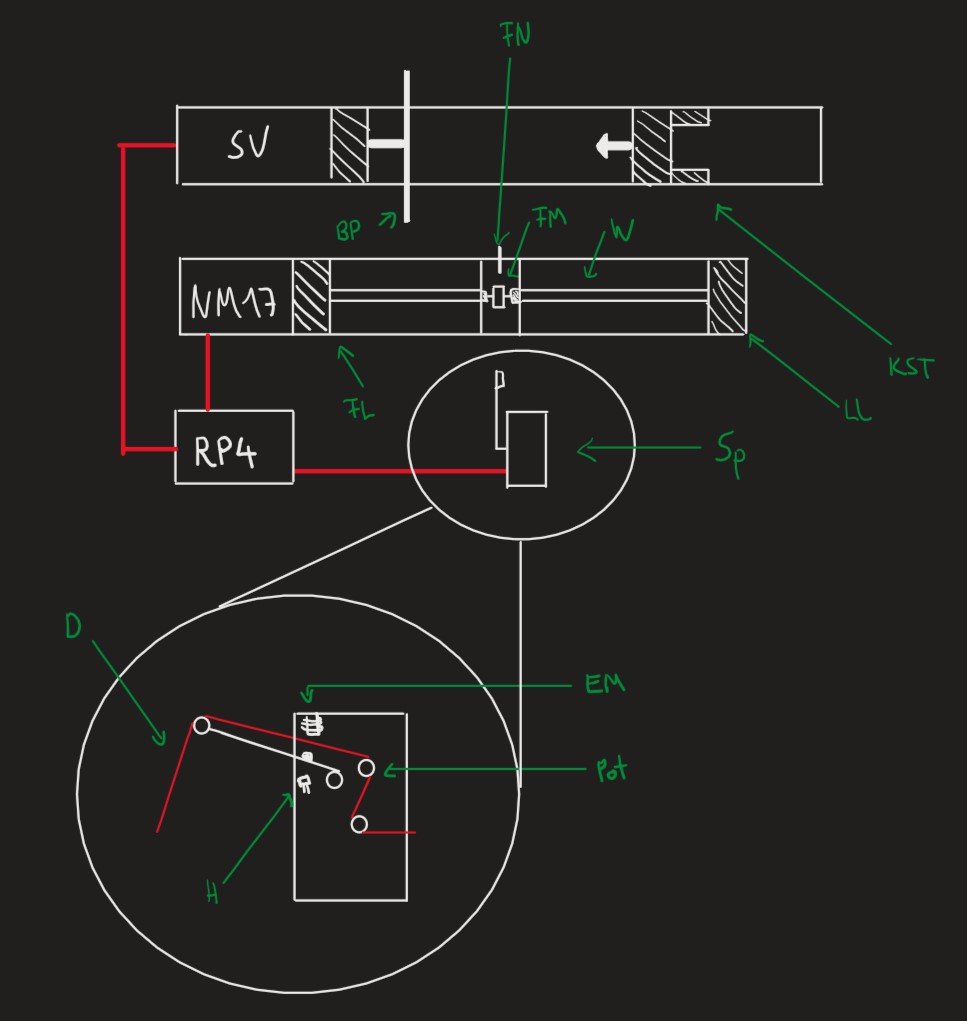
\includegraphics[width=\linewidth]{skizze.jpg}
    \caption{
        Skizze des Coil-Winders und der magnetischen Spannvorrichtung.
        \textbf{SV}: Servomotor; 
        \textbf{NM17}: Steppermotor; 
        \textbf{BP}: Befestigungsplatte; 
        \textbf{FN}: Führungsspitze; 
        \textbf{FM}: Führungsmechanismus; 
        \textbf{RP4}: Raspberry Pi 4; 
        \textbf{W}: Welle; 
        \textbf{LL}: Loslager; 
        \textbf{FL}: Festlager.
        \textbf{KST}: Konterreitstock;
        \textbf{SP}: Spannsystem;
        \textbf{EM}: Elektromagneten;
        \textbf{Pot}: Potentiometer;
        \textbf{H}: Hallsensor;
        \textbf{D}: Draht;
    }
\end{figure}


\section*{Physikalische/Hardware Anforderungen}
\begin{enumerate}
    \item mechanische Steifigkeit und Genauigkeit der Konstruktion.
    \item Ermittlung der Wirkkraft des magnetischen Spannsystems.
    \item Schnelle Schaltzeiten für das Schalten der Steppermotoren.
    \item Auflösungziel: $\Delta l =$ 0,05~mm.
\end{enumerate}


\section*{Komponenten und Kosten}
\begin{table}[H]
    \centering
    \caption{
        Skizze
    }
    \begin{tabular}{| c | c |}
        \hline
        Komponente &  Kosten / \euro{}\\
        \hline
        NEMA 17 (closed loop)& 15 - 60  \\
        \hline
        Servo Motor & 15 - 60  \\
        \hline
        Stepper Driver & 6 - 10  \\
        \hline
        sonst. Mat. & 50 - 80 \\
        \hline
        Arduino & vorhanden \\
        \hline
        RP4 (oder Alternative) & vorhanden \\
        \hline
        \hline
        Summe & 86 - 210  \\
        \hline
    \end{tabular}
\end{table}



\section*{Software}
\begin{enumerate}
    \item Stepper- und Servo-Steuerung
    \item Magnetfeldsteuerung
    \item Datenanalyse, Kalibration (RP4 (oder Alternative), C/C++ und Python)
    \item Simulation der Wicklung
\end{enumerate}

\section*{Aufwandsabschätzung}
\begin{table}[H]
    \centering
    \caption{
        Skizze
    }
    \begin{tabular}{| c | c |}
        \hline
        Arbeitspaket &  Aufwand / h\\
        \hline
        Mechanik/Halterungen & 40 - 60  \\
        \hline
        Stepper Steuerung / ADC Messung & 34 - 50 \\
        \hline
        RP4 Datenanalyse & 10 - 20  \\
        \hline
        Kalibration & 25 - 30 \\
        \hline
        Debugging & 50 - 100 \\
        \hline
        Modellprogrammierung & 30 - 40 \\
        \hline
        Mechanisches Testen & 5 - 15 \\
        \hline
        \hline
        Summe & 195 - 305  \\
        \hline
    \end{tabular}
    \label{tab:Aufwand}
\end{table}
        \printbibliography
    \end{multicols}
\end{document}